\documentclass[a4paper]{article}

\usepackage{pgfplots}

\pgfplotsset{compat=1.9}

\begin{document}

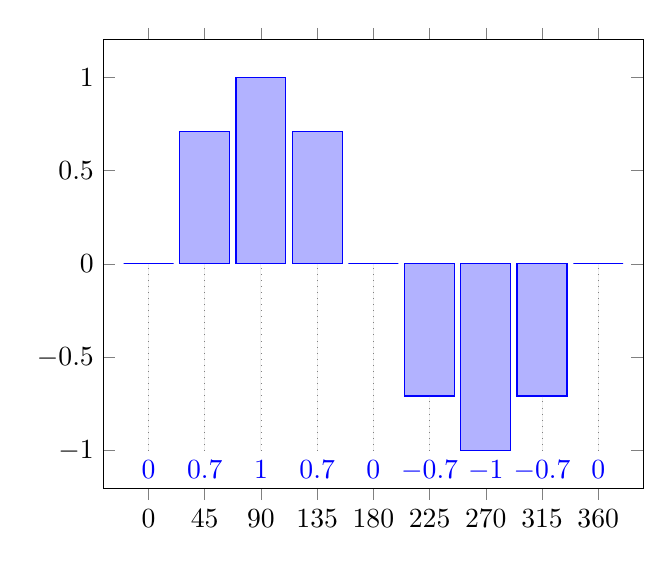
\begin{tikzpicture}
	\begin{axis}[
		ybar,
		bar width=360/9,
		nodes near coords,
		scatter/position=absolute,
		/pgfplots/scatter/@post marker code/.add code={}{
			\draw[dotted,help lines] (nodenearcoord\pgfkeysvalueof{/data point/index}) 
				-- (axis cs:\pgfkeysvalueof{/data point/x},{min(0,\pgfkeysvalueof{/data point/y})});
		},
		every node near coord/.code={
			\pgfkeysalso{
				name=nodenearcoord\pgfkeysvalueof{/data point/index},
				at={(axis cs:\pgfkeysvalueof{/data point/x},-1)},
				anchor=north,
				/pgf/number format/fixed,
				/pgf/number format/precision=1,
			}%
		},
		xtick=data,
	]
	\addplot+[domain=0:360,samples=9]
		{sin(x)};
	\end{axis}
\end{tikzpicture}

\end{document}

